\documentclass[conference]{IEEEtran}
%\IEEEoverridecommandlockouts

% Citings are in the 

\usepackage{cite}
\usepackage{amsmath,amssymb,amsfonts}
\usepackage{algorithmic}
\usepackage{graphicx}
\usepackage{textcomp}
\usepackage{xcolor}

\graphicspath{ {./img/} }

\def\BibTeX{{\rm B\kern-.05em{\sc i\kern-.025em b}\kern-.08em
    T\kern-.1667em\lower.7ex\hbox{E}\kern-.125emX}}

\begin{document}

\title{Security in WebRTC Peer-To-Peer networks and knowing who you're talking to\\
}

\author{\IEEEauthorblockN{Marc André Matija}
\IEEEauthorblockA{\textit{info@casqan.net}} \\
\textit{}
}

\maketitle

\begin{abstract}
\end{abstract}

\begin{IEEEkeywords}
peer-to-peer, WebRTC, WebSockets
\end{IEEEkeywords}

\section{Introduction}

HTTPs lock icon is not an indicator for security in modern browsers, as it only considers the HTTPs connection. \cite{BrowserToBrowserSecurity}
Any person can acquire an ssl certificate through the use of free services, such as Let's Encrypt %[https://letsencrypt.org/de/getting-started/]
and in the modern era, through corona and the rise of video-conferencing software such as Zoom or Big Blue Button, 
security in peer-to-peer becomes evermore important. As WebRTC Security poses different security concerns than
traditional Server-to-Client architectures I take a dive into the concerns and solutions to said challenges.
Although frequently used in other fields such as medical IOT infrastructure, to facilitate direct communication between
doctor and patient equipment.  

\section{Technical Background}
A prominent use for peer-to-peer technology is Web Real-Time Communication (WebRTC), a robust open-source framework that enables direct peer-to-peer 
communication between web browsers and other devices. With applications ranging from video conferencing 
to file sharing, WebRTC provides a low-latency, real-time communication framework integrated into modern 
browsers. Its implementation leverages standard protocols and APIs, offering developers seamless access to 
audio, video, and data transmission capabilities. % W3C. WebRTC 1.0: Real-time Communication Between Browsers. https://w3.org/TR/webrtc
WebRTC was initiated by Google in 2011 and is designed to enable web applications and sites to capture and optionally 
stream audio, video, and data between browsers or other endpoints without requiring external plugins.
The core protocols of WebRTC are standardized by the Internet Engineering Task Force (IETF), while the API specifications 
are defined by the World Wide Web Consortium (W3C). Together, they ensure interoperability across different platforms and devices.

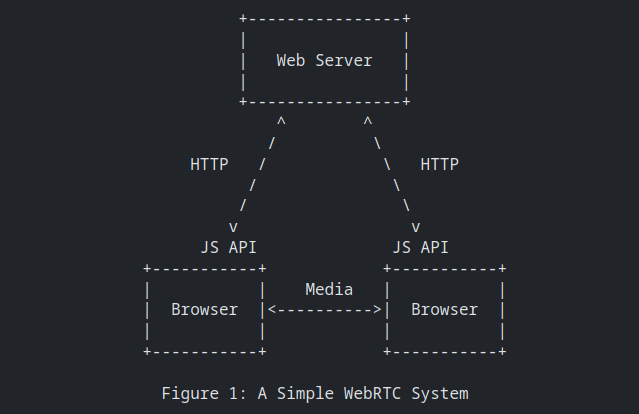
\includegraphics[width=0.45\textwidth]{WebRTC basic Structure}

Unlike most conventional real-time systems (e.g., SIP-based [RFC3261] soft phones), WebRTC 
communications are directly controlled by some Web server, via a JavaScript (JS) API as shown in Figure 1.


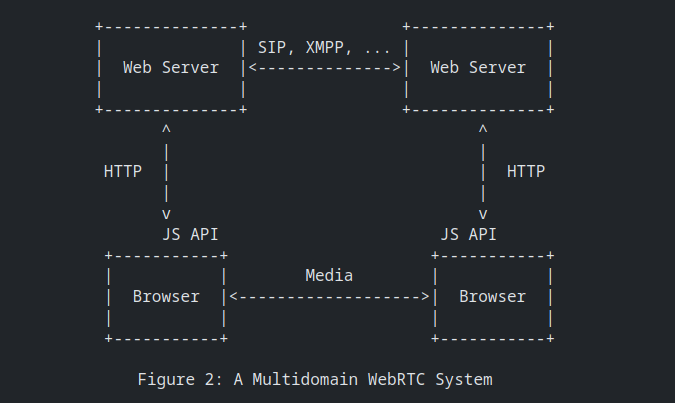
\includegraphics[width=0.45\textwidth]{multi domain calling.png}
A more complicated system might alow for inter-domain calling, as shown in Figure 2. The protocol to be used between the domains 
is not standardized by WebRTC, requires other form of security and may rely on other standardized Protocols such as the
Session initiation Protocol (SIP), or Extensible Messaging and Presence Protocol (XMPP) [RFC8827 1.1]

\section{Authentication in WebRTC}
\subsection{Trust Model}

The basic assumption of the standardized architecture as in RFC[8827] is that network resources exist in a hierarchy of trust, rooted in the browser, 
which serves as the user's Trusted Computing Base (TCB). Any security property which the user wishes to have enforced must be 
ultimately guaranteed by the browser (or transitively by some property the browser verifies). Conversely, if the browser is 
compromised, then no security guarantees are possible. Note that there are cases (e.g., Internet kiosks) where the user can't 
really trust the browser that much. In these cases, the level of security provided is limited by how much they trust the browser.
Optimally, we would not rely on trust in any entities other than the browser. However, this is unfortunately not possible 
if we wish to have a functional system. Other network elements fall into two categories: those which can be authenticated by 
the browser and thus can be granted permissions to access sensitive resources, and those which cannot be authenticated and 
thus are untrusted.

\subsection{Authenticated Entities}

There are two major classes of authenticated entities in the system:

Calling services:
    Web sites whose origin we can verify (optimally via HTTPS, but in some cases because we are on a topologically restricted 
    network, such as behind a firewall, and can infer authentication from firewall behavior).

Other users:
    WebRTC peers whose origin we can verify cryptographically (optimally via DTLS-SRTP).

Note that merely being authenticated does not make these entities trusted. For instance, just because we can verify that 
<https://www.example.org/> is owned by Dr. Evil does not mean that we can trust Dr. Evil to access our camera and microphone. 
However, it gives the user an opportunity to determine whether they wish to trust Dr. Evil or not; after all, if they desire to 
contact Dr. Evil (perhaps to arrange for ransom payment), it's safe to temporarily give them access to the camera and microphone 
for the purpose of the call, but they don't want Dr. Evil to be able to access their camera and microphone other than during the 
call. The point here is that we must first identify other elements before we can determine whether and how much to trust them.
 Additionally, sometimes we need to identify the communicating peer before we know what policies to apply.

\section{Identification in WebRTC}
Identification in Peer-To-Peer systems becomes a big problem, as a peer has to trust,
that a connecting peer is who he pretends to be. In the standard HTTPs environment the ssl
protocol is used to facilitate a trusted connection from client to server, in which the Server
has been previously verified by a Certificate Authority, which is trusted by the client. 
In a general sense, this means that two peers require a third trusted party to facilitate
identification in a secure manner. This part could be a peer, or superpeer that has been previously verified
by the opposing party and himself[]. % security Mechanisms for signaling in WebRTC-Based Peer-to-Peer Networks

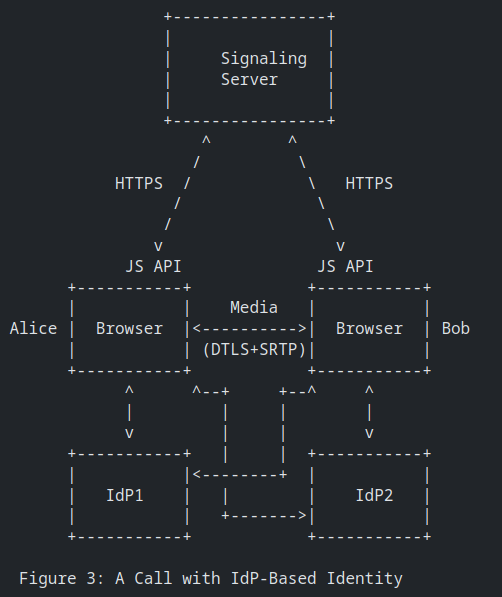
\includegraphics[width=0.45\textwidth]{call with IdP Based Identity.png}


\subsection{IdP}
As a standardized way, WebRTC offers and answers (and hence the channels established by
RTCPeerConnection objects) can be authenticated by using a web-based Identity
Provider (IdP). The idea is that the entity sending an offer or answer acts as the
Authenticating Party (AP) and obtains an identity assertion from the IdP which it
attaches to the session description. The consumer of the session description (i.e.,
the RTCPeerConnection on which setRemoteDescription is called) acts as the
Relying Party (RP) and verifies the assertion. % Identity for WebRTC 1.0 https://www.w3.org/TR/webrtc-identity/

In order to verify assertions, the IdP domain name and protocol are taken from the
domain and protocol fields of the identity assertion.

Communication with the IdP is established by the user agent loading the IdP JavaScript from
the IdP. The URI for the IdP script is a well-known URI formed from the “domain”
and “protocol” fields, as specified in [RTCWEB-SECURITY-ARCH].
The IdP MAY generate an HTTP redirect to another "https" origin, the browser
MUST treat a redirect to any other scheme as a fatal error.
The user agent instantiates an isolated interpreted context, a JavaScript realm that
operates in the origin of the loaded JavaScript. Note that a redirect will change the
origin of the loaded script.
The realm is populated with a global that implements both the
RTCIdentityProviderGlobalScope and WorkerGlobalScope [WEBWORKERS]
interfaces.
The user agent provides an instance of RTCIdentityProviderRegistrar named
rtcIdentityProvider in the global scope of the realm. This object is used by the IdP to
interact with the user agent.

An environment that mimics the identity provider realm can be provided by any
script. However, only scripts running in the origin of the IdP are able to generate an
identical environment. Other origins can load and run the IdP proxy code, but they
will be unable to replicate data that is unique to the origin of the IdP.
This means that it is critical that an IdP use data that is restricted to its own origin
when generating identity assertions. Otherwise, another origin could load the IdP
script and use it to impersonate users.
The data that the IdP script uses could be stored on the client (for example, in
[INDEXEDDB]) or loaded from servers. Data that is acquired from a server SHOULD
require credentials and be protected from cross-origin access.
There is no risk to the integrity of identity assertions if an IdP validates an identity
assertion without using origin-private data.

This assertions is standardized as the "identity" attribute, a session-level attribute that is used by an endpoint to 
convey its identity assertion to its peer. [RFC8827]
The procedures in this section are based on the assumption that the identity assertion 
of an endpoint is bound to the fingerprints of the endpoint. THe "identity" attribute
is not defined for multiple identities within it's field and implementations of WebRTC
should only include a single "identity" attribute, while relying parties may elect to
only trust the first "identity" attribute and ignore all other "identity" attributes
found in an sdp. [RFC8827]

\section{Authenticity and Data Integrity}
WebRTC at it's core uses User Datagram Protocol a lightweight, connectionless communication protocol 
within the Internet Protocol (IP) suite, defined in [RFC 768]. It enables applications to send and receive 
discrete packets of data, known as datagrams, without requiring a prior connection. While UDP, does
include a checksum to verify it's data integrity, it does not include any standard specification for ensuring
packages have been received by the opposing party, relying on protocol extensions to facilitate save
data transmission.
WebRTC enforces end-to-end encryption for all media and data streams by default, using 
standards like DTLS for signaling and data channels while relying on SRTP for media transmission. [RFC8826]
protocol is a cryptographic protocol designed to provide secure communication over unreliable datagram-based 
transport layers such as UDP. It is defined in RFC 6347 and serves as an adaptation of the widely used Transport 
Layer Security (TLS) protocol, which secures communication over connection-oriented transport protocols like TCP. 
By incorporating mechanisms to handle packet loss, reordering, and duplication, DTLS ensures secure, reliable 
communication in real-time and low-latency scenarios. % rfc6347

% \section{WebRTC and Chord}
% . Chord
% Chord [1] is a common structured P2P network protocol
% which forms a Distributed Hash Table (DHT) for organizing
% peers and data items.  $ P = \{ p_1,...,p_N \}$ is a set of N peers
% and $D = \{d_1, . . . , d_L\}$  is a set of L data items. Chord
% employs a cryptographic hash function H : {0, 1}* → {0, 1}n
% to compute a fixed length identifier (ID) of n bits for every
% peer $p_i \in P $ and every data item $d_k \in D$. The identifiers are
% denoted as hpi and hdk , respectively. Based on their identifiers,
% which are called keys for data items, all peers are arranged in
% a ring, the so-called Chord-ring. Subsequently, peer pi is in
% charge of data items in the key space between the predecessor’s
% ID and its own ID: ( hpred(pi), hpi ].
% Chord’s core operation is to find pi, which is in charge of
% a given hash value hx: pi = find successor(hx). Since every
% peer knows how to contact its successor, this operation can
% be na¨ıvely implemented by walking along the ring of peers in
% O(N ) steps (see Figure 2). For scalability, Chord improves the
% inefficient lookup to log2(N ) steps. Since this is not required
% for our approach, we refer the interested reader to [1].
% One can use Chord to store and retrieve key-value pairs,
% where data items are the values and hashes are their corre-
% sponding keys: put(hd, d) and d = get(hd).

\section{Challenges and Future Directions}

Highlighted in the paper One leak will sink the ship, WebRTC's strength can also be it's biggest
problem. Due to it's inherent nature of establishing a Peer-To-Peer connection, WebRTC requires
knowledge about a peers ip address, cause the potential leak of someone's location, even with
the use of VPN's. Possible leaked information can include the users 
\begin{itemize}
    \item \it{Public IPv6 address} this is the IPv6 address of the
    platform and is typically assigned by the ISP of the client.
    \item \it{Public Temporary IPv6 address:} this address is assigned
    by the network to which the client platform is attached.
    \item \it{Unique local address (ULA) assigned by LAN:} this IPv6
    address is assigned by the network to which the client
    platform is attached, and is the approximate IPv6 coun-
    terpart of the Private IPv4 address assigned by LAN [5].
    \item \it{Private IP address assigned by the VPN server:} this pri-
    vate (IPv4 or IPv6, depending on the VPN configuration)
    address is assigned by the VPN server.
    \item \it{Private IPv4 address assigned by LAN:} this address is 
    assigned by the network to which the client platform is
    attached.
  \end{itemize} % IP address leaks -> One leak will sink a ship
While not all of these are worth the same, a public IPv6 Address leak for example, is more dangerous than a
Unique local Address leak, these are still security concerns VPNs try to solve.
VPN providers have now setup WebRTC address leak detectors to inform the user, if a leak of their private IP address
is present. Providers for these Services include some of the major players in the private VPN space, such as 
[ExpressVPN] and [Surfshark] % https://www.expressvpn.com/webrtc-leak-test 
Some solutions to this problem include:
\begin{itemize}
    \item Disabling WebRTC entirely inside the Browser or connecting client.
    \item Disabling IPv6 to reduce the amount of information leaked, if a leak occurs.
    \item Relying on Relay Server to transmit data to a central location before continuing on to the connected peer,
    which however, does need to be implemented by the Developers of the application using WebRTC, which defeats the
    purpose of not having a central server in peer-to-peer to begin with.
\end{itemize} % IP address leaks -> One leak will sink a ship
as outlined in [1].
However, all these are mere workarounds and WebRTC without VPNs has to inherently leak
IP addresses as they are required to connect to another peer.


\section{Conclusion}

\begin{thebibliography}{00}
    \bibitem{paper} 
\end{thebibliography}

\end{document}